\section*{Decremental Consistency Checking Problem}

\begin{frame}{Constraint Satisfactory Problem (\CSPName)}
    \begin{block}{Constraint Satisfactory Problem (\CSPName{})}%
		A CSP $\CSP{}$ consists of a finite set of \textit{variables} $\mathcal{V} = \{ x_1, x_2, ... x_n \}$; 
        each variable $x \in \mathcal{V}$ has associated a finite domain of values $Dom(x) = \{ v_1, ..., v_k\}$ and a finite set of constraints $\mathcal{C} = \{ C_1, ..., C_m \}$.
	\end{block}

    Example: Graph coloring

    \begin{minipage}{0.28\textwidth}
        \begin{figure}
            \centering
            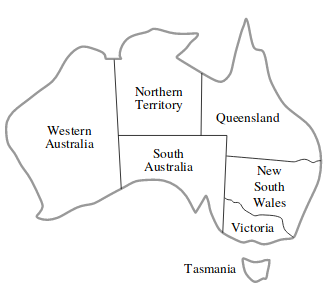
\includegraphics[width=1.0\textwidth]{{{src/images/temporal-reasoning/australia-map}}}
        \end{figure}
    \end{minipage}\hfill%
    \begin{minipage}{0.68\textwidth}
        \begin{equation*}
            \begin{split}
                \mathcal{V} & = \{ WA, NT, SA, Q, NSW, V, T \} \\
                Dom(x) & = \{ red, green, blue \}, \forall x \in \mathcal{V} \\
                \mathcal{C} & = \{ SA \not = WA, SA \not = NT, SA \not = Q, \\
                & \;\;\;\; SA \not = NSW, SA \not = V, \\
                & \;\;\;\; WA \not = NT, NT \not = Q, Q \not = NSW, \\
                & \;\;\;\; NSW \not = V \}
            \end{split}
        \end{equation*}
    \end{minipage}

\end{frame}

\begin{frame}{Constraint Graph}
    \CSPNames{} can be represented via \textit{constraint graphs}. 
    A \textit{solution} is a complete assignment of the variables which satisfies \textbf{all} constraints.

    \vspace{-8pt}
    \begin{minipage}{0.23\textwidth}
        \centering
        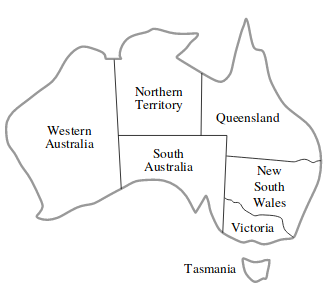
\includegraphics[width=1.0\textwidth]{{{src/images/temporal-reasoning/australia-map}}}
    \end{minipage}\hfill%
    \begin{minipage}{0.75\textwidth}
        \begin{equation*}
            \begin{split}
                \mathcal{V} & = \{ WA, NT, SA, Q, NSW, V, T \} \\
                Dom(x) & = \{ red, green, blue \}, \forall x \in \mathcal{V} \\
                \mathcal{C} & = \{ SA \not = WA, SA \not = NT, SA \not = Q, \\
                & \;\;\;\; SA \not = NSW, SA \not = V, WA \not = NT, \\
                & \;\;\;\; NT \not = Q, Q \not = NSW, NSW \not = V \}
            \end{split}
        \end{equation*}
    \end{minipage}\\
    \begin{minipage}{0.5\textwidth}
        \begin{figure}
            \centering
            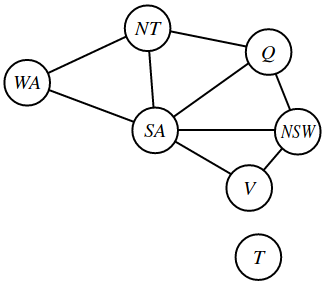
\includegraphics[width=0.5\textwidth]{src/images/temporal-reasoning/australia-graph}
            \caption{Constraint graph of \CSP{}.}
        \end{figure}
    \end{minipage}\hfill%
    \begin{minipage}{0.5\textwidth}
        \begin{figure}
            \centering
            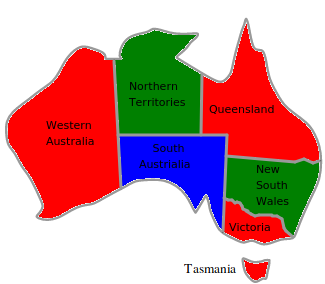
\includegraphics[width=0.5\textwidth]{src/images/temporal-reasoning/australia-map-colored}
            \caption{Representation of a solution of \CSP{}.}
        \end{figure}
    \end{minipage}
\end{frame}

\begin{frame}{Consistency}
    \begin{block}{Consistency}
		A CSP $\CSP{}$ is \textbf{satisfiable} (\textbf{consistent}) iff there is at least one solution 
        (\ie{} assignment of values to all the variables $\{x_i = v_i\}$ s.t. no constraint is violated).
	\end{block}

    \begin{figure}
        \centering
        \begin{subfigure}{0.48\textwidth}
            \centering
            \begin{tikzpicture}
                \tikzstyle{vertex} = [shape=circle, fill=blue!20, draw=blue!50, thick, minimum size=2mm, inner sep=5pt, distance=1.7cm];

                \node[vertex](X) at (23:0.9cm) {$x$};
                \node[vertex](Y) at (113:0.9cm) {$y$};
                \node[vertex](Z) at (203:0.9cm) {$z$};
                \node[vertex](T) at (293:0.9cm) {$t$};

                \draw[-{Latex[length=2mm,width=3mm]}, line width=0.3mm]
                    (X) edge node[above]{$<$} (Y)
                    (Y) edge node[left]{$<$} (Z)
                    (Z) edge node[below]{$<$} (T)
                ;
            \end{tikzpicture}
            \caption{Constraint graph of a consistent \CSPName{}}
        \end{subfigure}\hfill%
        \begin{subfigure}{0.48\textwidth}
            \centering
            \begin{tikzpicture}
                \tikzstyle{vertex} = [shape=circle, fill=blue!20, draw=blue!50, thick, minimum size=2mm, inner sep=5pt, distance=1.7cm];

                \node[vertex](X) at (23:0.9cm) {$x$};
                \node[vertex](Y) at (113:0.9cm) {$y$};
                \node[vertex](Z) at (203:0.9cm) {$z$};
                \node[vertex](T) at (293:0.9cm) {$t$};

                \draw[-{Latex[length=2mm,width=3mm]}, line width=0.3mm]
                    (X) edge[color=red] node[above]{$<$} (Y)
                    (Y) edge[color=red] node[left]{$<$} (Z)
                    (Z) edge[color=red] node[below]{$<$} (X)
                    (Z) edge node[below]{$<$} (T)
                ;
            \end{tikzpicture}
            \caption{Constraint graph of an inconsistent \CSPName{}}
        \end{subfigure}
    \end{figure}

\end{frame}

\begin{frame}{Temporal \CSPNames{}}
    \begin{itemize}
        \item Focus on \TCSPNames{} (\ie{} \CSPNames{} where the variables represent timed events and each constraint involves a relation between 2 events);
        \item constraints: relations in Point Algebra (\PAName{}), Interval Algebra (\IAName{}) or its maximal tractable subalgebra,  \OrdHornName{}.
        \item variables: time points (for \PAName{}) or time intervals (for \IAName{});
        \item \IAName{}: $\bot$, 13 base relations and all their possible unions (\eg{} two intervals cannot overlap);
        \item \PAName{}: $<, =, >, \leq, \geq, \noteq{}, \top, \bot$ (\eg{} $x \noteq{} y$ means that the two events cannot occur at the same time); example of a \TCSPName{} over \PAName{}:
	\end{itemize}

    \begin{figure}
        \centering
        \begin{subfigure}{0.44\textwidth}
            \centering
            \begin{tikzpicture}
                \tikzstyle{vertex} = [shape=circle, fill=blue!20, draw=blue!50, thick, minimum size=2mm, inner sep=5pt, distance=1.7cm];

                \node[vertex](X) at (23:0.9cm) {$x$};
                \node[vertex](Y) at (113:0.9cm) {$y$};
                \node[vertex](Z) at (203:0.9cm) {$z$};
                \node[vertex](T) at (293:0.9cm) {$t$};

                \draw[-{Latex[length=2mm,width=3mm]}, line width=0.3mm]
                    (X) edge node[above]{$<$} (Y)
                    (Y) edge node[left]{$\geq$} (Z)
                ;

                \draw[-., line width=0.3mm]
                    (Z) edge node[below]{$\noteq{}$} (T)
                    (X) edge node[right]{$=$} (T)
                ;
            \end{tikzpicture}
        \end{subfigure}\hfill%
        \begin{subfigure}{0.1\textwidth}
            \centering
            $\xrightarrow{\mbox{\tlGraphName{}}}$
        \end{subfigure}\hfill%
        \begin{subfigure}{0.44\textwidth}
            \centering
            \begin{tikzpicture}
                \tikzstyle{vertex} = [shape=circle, fill=blue!20, draw=blue!50, thick, minimum size=2mm, inner sep=5pt, distance=1.7cm];

                \node[vertex](X) at (23:0.9cm) {$x$};
                \node[vertex](Y) at (113:0.9cm) {$y$};
                \node[vertex](Z) at (203:0.9cm) {$z$};
                \node[vertex](T) at (293:0.9cm) {$t$};

                \draw[-{Latex[length=2mm,width=3mm]}, line width=0.3mm]
                    (X) edge node[above]{$<$} (Y)
                    (Z) edge node[left]{$\leq$} (Y)
                    (X) edge[bend left] node[right]{$\leq$} (T)
                    (T) edge[bend left] node[left]{$\leq$} (X)
                ;

                \draw[-., line width=0.3mm]
                    (Z) edge node[below]{$\noteq{}$} (T)
                ;
            \end{tikzpicture}
        \end{subfigure}
    \end{figure}
\end{frame}